\subsection{Planar data classification with a hidden layer}

Welcome to the second programming exercise of the deep learning specialization. In this notebook you will generate red and blue points to form a flower. You will then fit a neural network to correctly classify the points. You will try different layers and see the results.

\begin{figure}[h]
\begin{center}

\includegraphics[width=\textwidth]{course1/Hidden_Layer}
\end{center}
\caption{classify points}
\label{fig:Hidden_Layer}
\end{figure}

By completing this assignment you will:
\begin{itemize}
\item Develop an intuition of back-propagation and see it work on data.
\item Recognize that the more hidden layers you have the more complex structure you could capture.
\item Build all the helper functions to implement a full model with one hidden layer.
\end{itemize}


You will learn how to:
\begin{itemize}
\item Implement a 2-class classification neural network with a single hidden layer
\item Use units with a non-linear activation function, such as tanh
\item Compute the cross entropy loss
\item Implement forward and backward propagation
\end{itemize}

This assignment prepares you well for the upcoming assignment. Take your time to complete it and make sure you get the expected outputs when working through the different exercises. In some code blocks, you will find a "\#GRADED FUNCTION: functionName" comment. Please do not modify it. After you are done, submit your work and check your results. You need to score 70\% to pass. Good luck :) !


\subsubsection{Packages}

Let's first import all the packages that you will need during this assignment.
\begin{itemize}
\item \href{http://www.numpy.org/}{numpy} is the fundamental package for scientific computing with Python.
\item \href{http://scikit-learn.org/stable/}{sklearn} provides simple and efficient tools for data mining and data analysis.
\item \href{https://matplotlib.org/}{matplotlib} is a library for plotting graphs in Python.
\item testCases provides some test examples to assess the correctness of your functions
\item planar\_utils provide various useful functions used in this assignment
\end{itemize}

\begin{minted}{python}
# Package imports
import numpy as np
import matplotlib.pyplot as plt
from testCases_v2 import *
import sklearn
import sklearn.datasets
import sklearn.linear_model
from planar_utils import plot_decision_boundary, sigmoid, load_planar_dataset, load_extra_datasets

#matplotlib inline

np.random.seed(1) # set a seed so that the results are consistent
\end{minted}

\subsubsection{Dataset}

First, let's get the dataset you will work on. The following code will load a "flower" 2-class dataset into variables X and Y.
\begin{minted}{python}
X, Y = load_planar_dataset()
\end{minted}

Visualize the dataset using matplotlib. The data looks like a "flower" with some red (label y=0) and some blue (y=1) points. Your goal is to build a model to fit this data.
\begin{minted}{python}
# Visualize the data:
plt.scatter(X[0, :], X[1, :], c=Y, s=40, cmap=plt.cm.Spectral);
\end{minted}

\begin{figure}[h]
\begin{center}
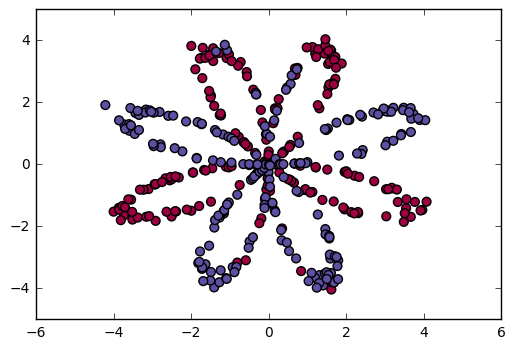
\includegraphics[width=0.6\textwidth]{course1/visualize_data}
\end{center}
\caption{Visualize the dataset}
\label{fig:visualize_data}
\end{figure}


You have:
\begin{itemize}
\item a numpy-array (matrix) X that contains your features (x1, x2)
\item a numpy-array (vector) Y that contains your labels (red:0, blue:1).
\end{itemize}

Lets first get a better sense of what our data is like.

{\textbf{Exercise}}: How many training examples do you have? In addition, what is the shape of the variables X and Y?

\begin{minted}{python}
### START CODE HERE ### (≈ 3 lines of code)
shape_X = X.shape
shape_Y = Y.shape
m = shape_X[1]  # training et size
### END CODE HERE ###

print ('The shape of X is: ' + str(shape_X))
print ('The shape of Y is: ' + str(shape_Y))
print ('I have m = %d training examples.' % (m))

#output
The shape of X is: (2, 400)
The shape of Y is: (1, 400)
I have m = 400 training examples.
\end{minted}


\subsubsection{Simple Logistic Regression}

Before building a full neural network, lets first see how logistic regression performs on this problem. You can use sklearn's built-in functions to do that. Run the code below to train a logistic regression classifier on the dataset.
\begin{minted}{python}
# Train the logistic regression classifier
clf = sklearn.linear_model.LogisticRegressionCV();
clf.fit(X.T, Y.T);
\end{minted}

You can now plot the decision boundary of these models. Run the code below
\begin{minted}{python}
# Plot the decision boundary for logistic regression
plot_decision_boundary(lambda x: clf.predict(x), X, Y)
plt.title("Logistic Regression")

# Print accuracy
LR_predictions = clf.predict(X.T)
print ('Accuracy of logistic regression: %d ' % float((np.dot(Y,LR_predictions) + np.dot(1-Y,1-LR_predictions))/float(Y.size)*100) +
       '% ' + "(percentage of correctly labelled datapoints)")
\end{minted}


The result is as follows:
\begin{minted}{python}
Accuracy of logistic regression: 47 % (percentage of correctly labelled datapoints)
\end{minted}
\begin{figure}[h]
\begin{center}
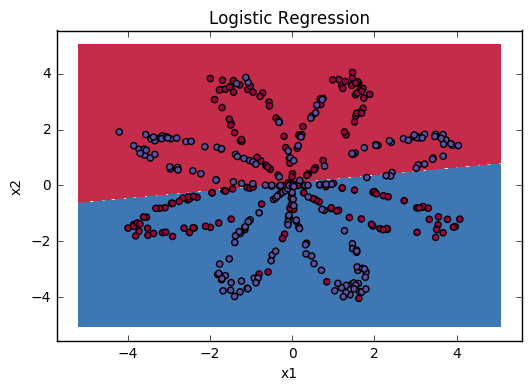
\includegraphics[width=0.6\textwidth]{course1/Logistic_Regression}
\end{center}
\caption{Logistic Regression}
\label{fig:Logistic_Regression}
\end{figure}

{\textbf {Interpretation}}: The dataset is not linearly separable, so logistic regression doesn't perform well. Hopefully a neural network will do better. Let's try this now!

\subsubsection{Neural Network model}

Logistic regression did not work well on the "flower dataset". You are going to train a Neural Network with a single hidden layer.

Here is our model:
\begin{figure}[h]
\begin{center}
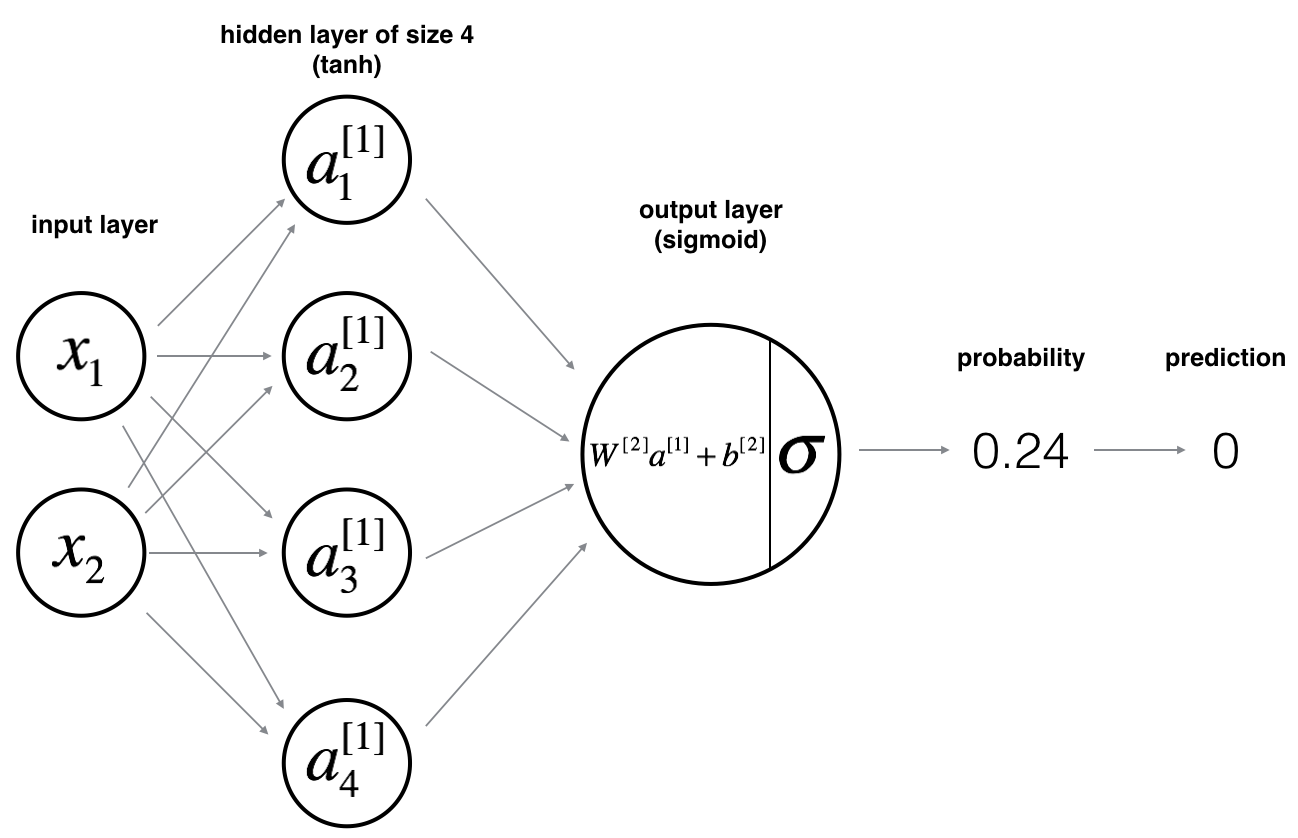
\includegraphics[width=0.6\textwidth]{course1/Neural_Network_model}
\end{center}
\caption{Neural Network Model}
\label{fig:Neural_Network_model}
\end{figure}

{\textbf {Mathematically}}:

For one example $x^{(i)}$:
\begin{align}
z^{[1] (i)} &=  W^{[1]} x^{(i)} + b^{[1] (i)}\\
a^{[1] (i)} &= \tanh(z^{[1] (i)})\\
z^{[2] (i)} &= W^{[2]} a^{[1] (i)} + b^{[2] (i)}\\
\hat{y}^{(i)} &= a^{[2] (i)} = \sigma(z^{ [2] (i)})\\
y^{(i)}_{prediction} &= \begin{cases} 1 & \mbox{if } a^{[2](i)} > 0.5 \\ 0 & \mbox{otherwise } \end{cases}
\end{align}

Given the predictions on all the examples, you can also compute the cost $J$ as follows:
\begin{align}
J = - \frac{1}{m} \sum\limits_{i = 0}^{m} \large\left(\small y^{(i)}\log\left(a^{[2] (i)}\right) + (1-y^{(i)})\log\left(1- a^{[2] (i)}\right)  \large  \right) \small 
\end{align}



{\textbf {Reminder}}: The general methodology to build a Neural Network is to:
\begin{itemize}
\item[1] Define the neural network structure ( \# of input units,  \# of hidden units, etc). 
\item[2] Initialize the model's parameters
\item[3] Loop:
\begin{itemize}
\item Implement forward propagation
\item Compute loss
\item Implement backward propagation to get the gradients
\item Update parameters (gradient descent)
\end{itemize}
\end{itemize}

You often build helper functions to compute steps 1-3 and then merge them into one function we call `nn\_model()'. Once you've built `nn\_model()' and learnt the right parameters, you can make predictions on new data.


\subsubsubsection{Defining the neural network structure}\label{section4.1}

{\textbf {Exercise}}: Define three variables:
\begin{itemize}
\item n\_x: the size of the input layer
\item n\_h: the size of the hidden layer (set this to 4) 
\item n\_y: the size of the output layer
\end{itemize}

{\textbf {Hint}}: Use shapes of X and Y to find n\_x and n\_y. Also, hard code the hidden layer size to be 4.

\begin{minted}{python}
# GRADED FUNCTION: layer_sizes

def layer_sizes(X, Y):
    """
    Arguments:
    X -- input dataset of shape (input size, number of examples)
    Y -- labels of shape (output size, number of examples)
    
    Returns:
    n_x -- the size of the input layer
    n_h -- the size of the hidden layer
    n_y -- the size of the output layer
    """
    ### START CODE HERE ### (≈ 3 lines of code)
    n_x = X.shape[0] # size of input layer
    n_h = 4
    n_y = Y.shape[0]# size of output layer
    ### END CODE HERE ###
    return (n_x, n_h, n_y)
\end{minted}



\subsubsubsection{Initialize the model's parameters}\label{section4.2}

{\textbf {Exercise}}: Implement the function initialize\_parameters().

{\textbf {Instructions}}:
\begin{itemize}
\item Make sure your parameters' sizes are right. Refer to the neural network figure above if needed.
\item You will initialize the weights matrices with random values.
\begin{itemize}
\item Use: np.random.randn(a,b) * 0.01 to randomly initialize a matrix of shape (a,b).
\end{itemize}
\item You will initialize the bias vectors as zeros.
\begin{itemize}
\item Use: np.zeros((a,b)) to initialize a matrix of shape (a,b) with zeros.
\end{itemize}
\end{itemize}

\begin{minted}{python}
# GRADED FUNCTION: initialize_parameters

def initialize_parameters(n_x, n_h, n_y):
    """
    Argument:
    n_x -- size of the input layer
    n_h -- size of the hidden layer
    n_y -- size of the output layer
    
    Returns:
    params -- python dictionary containing your parameters:
                    W1 -- weight matrix of shape (n_h, n_x)
                    b1 -- bias vector of shape (n_h, 1)
                    W2 -- weight matrix of shape (n_y, n_h)
                    b2 -- bias vector of shape (n_y, 1)
    """
    
    np.random.seed(2) # we set up a seed so that your output matches ours although the initialization is random.
    
    ### START CODE HERE ### (≈ 4 lines of code)
    W1 = np.random.randn(n_h,n_x) * 0.01
    b1 = np.zeros((n_h,1))
    W2 = np.random.randn(n_y,n_h)* 0.01
    b2 = np.zeros((n_y,1))
    ### END CODE HERE ###
    
    assert (W1.shape == (n_h, n_x))
    assert (b1.shape == (n_h, 1))
    assert (W2.shape == (n_y, n_h))
    assert (b2.shape == (n_y, 1))
    
    parameters = {"W1": W1,
                  "b1": b1,
                  "W2": W2,
                  "b2": b2}
    
    return parameters
\end{minted}



\subsubsubsection{The Loop}\label{section4.3}


{\textbf {Question}}: Implement `forward\_propagation()'.

{\textbf {Instructions}}:
\begin{itemize}
\item Look above at the mathematical representation of your classifier.
\item You can use the function `sigmoid()'. It is built-in (imported) in the notebook.
\item You can use the function `np.tanh()'. It is part of the numpy library.
\item The steps you have to implement are:
\begin{itemize}
    \item[1] Retrieve each parameter from the dictionary ``parameters" (which is the output of `initialize\_parameters()') by using `parameters[``.."]'.
    \item[2] Implement Forward Propagation. Compute $Z^{[1]}, A^{[1]}, Z^{[2]}$ and $A^{[2]}$ (the vector of all your predictions on all the examples in the training set).
\end{itemize}    
\item Values needed in the backpropagation are stored in ``cache". The \emph{cache} will be given as an input to the backpropagation function.
\end{itemize}



\begin{minted}{python}
# GRADED FUNCTION: forward_propagation

def forward_propagation(X, parameters):
    """
    Argument:
    X -- input data of size (n_x, m)
    parameters -- python dictionary containing your parameters (output of initialization function)
    
    Returns:
    A2 -- The sigmoid output of the second activation
    cache -- a dictionary containing "Z1", "A1", "Z2" and "A2"
    """
    # Retrieve each parameter from the dictionary "parameters"
    ### START CODE HERE ### (≈ 4 lines of code)
    W1 = parameters["W1"]
    b1 = parameters["b1"]
    W2 = parameters["W2"]
    b2 = parameters["b2"]
    ### END CODE HERE ###
    
    # Implement Forward Propagation to calculate A2 (probabilities)
    ### START CODE HERE ### (≈ 4 lines of code)
    Z1 = np.dot(W1,X)+b1
    A1 = np.tanh(Z1)
    Z2 = np.dot(W2,A1)+b2
    A2 = sigmoid(Z2)
    ### END CODE HERE ###
    
    assert(A2.shape == (1, X.shape[1]))
    
    cache = {"Z1": Z1,
             "A1": A1,
             "Z2": Z2,
             "A2": A2}
    
    return A2, cache
\end{minted}


Now that you have computed $A^{[2]}$ (in the Python variable ``A2"), which contains $a^{[2](i)}$ for every example, you can compute the cost function as follows:
\begin{equation}
J = - \frac{1}{m} \sum\limits_{i = 0}^{m} \large{(} \small y^{(i)}\log\left(a^{[2] (i)}\right) + (1-y^{(i)})\log\left(1- a^{[2] (i)}\right) \large{)} \small
\end{equation}

{\textbf {Exercise}}: Implement ``compute\_cost()'' to compute the value of the cost $J$.

{\textbf {Instructions}}:

There are many ways to implement the cross-entropy loss. To help you, we give you how we would have implemented
$- \sum\limits_{i=0}^{m}  y^{(i)}\log(a^{[2](i)})$:

\begin{minted}{python}
logprobs = np.multiply(np.log(A2),Y)
cost = - np.sum(logprobs)                # no need to use a for loop!
\end{minted}

(you can use either ``np.multiply()'' and then ``np.sum()'' or directly `np.dot()').

\begin{minted}{python}
# GRADED FUNCTION: compute_cost
def compute_cost(A2, Y, parameters):
    """
    Computes the cross-entropy cost given in equation (13)
    
    Arguments:
    A2 -- The sigmoid output of the second activation, of shape (1, number of examples)
    Y -- "true" labels vector of shape (1, number of examples)
    parameters -- python dictionary containing your parameters W1, b1, W2 and b2
    
    Returns:
    cost -- cross-entropy cost given equation (13)
    """
    
    m = Y.shape[1] # number of example

    # Compute the cross-entropy cost
    ### START CODE HERE ### (≈ 2 lines of code)
    logprobs = np.multiply(np.log(A2),Y)+np.multiply(np.log(1-A2),1-Y)
    cost = - np.sum(logprobs)/m
    ### END CODE HERE ###
#    use directly np.dot())
#    cost=-(np.dot(Y,np.log(A2.T))+np.dot(np.log(1-A2),(1-Y).T))/m
    
    cost = np.squeeze(cost)     # makes sure cost is the dimension we expect. 
                                # E.g., turns [[17]] into 17 
    
    return cost
\end{minted}


Using the cache computed during forward propagation, you can now implement {\textbf {backward propagatio}}.

{\textbf {Question}}: Implement the function backward\_propagation().

{\textbf {Instructions}}: Backpropagation is usually the hardest (most mathematical) part in deep learning. To help you, here again is the slide from the lecture on backpropagation. You'll want to use the six equations on the right of this slide, since you are building a vectorized implementation.

\begin{align}
\frac{\partial \mathcal{J} }{ \partial z_{2}^{(i)} } &= \frac{1}{m} (a^{[2](i)} - y^{(i)})\\
\frac{\partial \mathcal{J} }{ \partial W_2 } &= \frac{\partial \mathcal{J} }{ \partial z_{2}^{(i)} } a^{[1] (i) T} \\
\frac{\partial \mathcal{J} }{ \partial b_2 } &= \sum_i{\frac{\partial \mathcal{J} }{ \partial z_{2}^{(i)}}}
\end{align}
\begin{align}
\frac{\partial \mathcal{J} }{ \partial z_{1}^{(i)} } &=  W_2^T \frac{\partial \mathcal{J} }{ \partial z_{2}^{(i)} } * ( 1 - a^{[1] (i) 2}) \\
\frac{\partial \mathcal{J} }{ \partial W_1 } &= \frac{\partial \mathcal{J} }{ \partial z_{1}^{(i)} }  X^T \\
\frac{\partial \mathcal{J} _i }{ \partial b_1 } &= \sum_i{\frac{\partial \mathcal{J} }{ \partial z_{1}^{(i)}}}
\end{align}

\begin{itemize}
\item Note that $*$ denotes elementwise multiplication.
\item The notation you will use is common in deep learning coding:
\begin{itemize}
\item dW1 = $\frac{\partial \mathcal{J} }{ \partial W_1 }$
\item db1 = $\frac{\partial \mathcal{J} }{ \partial b_1 }$   
\item dW2 = $\frac{\partial \mathcal{J} }{ \partial W_2 }$   
\item db2 = $\frac{\partial \mathcal{J} }{ \partial b_2 }$
\end{itemize}    
\end{itemize} 
   

\begin{figure}[h]
\begin{center}
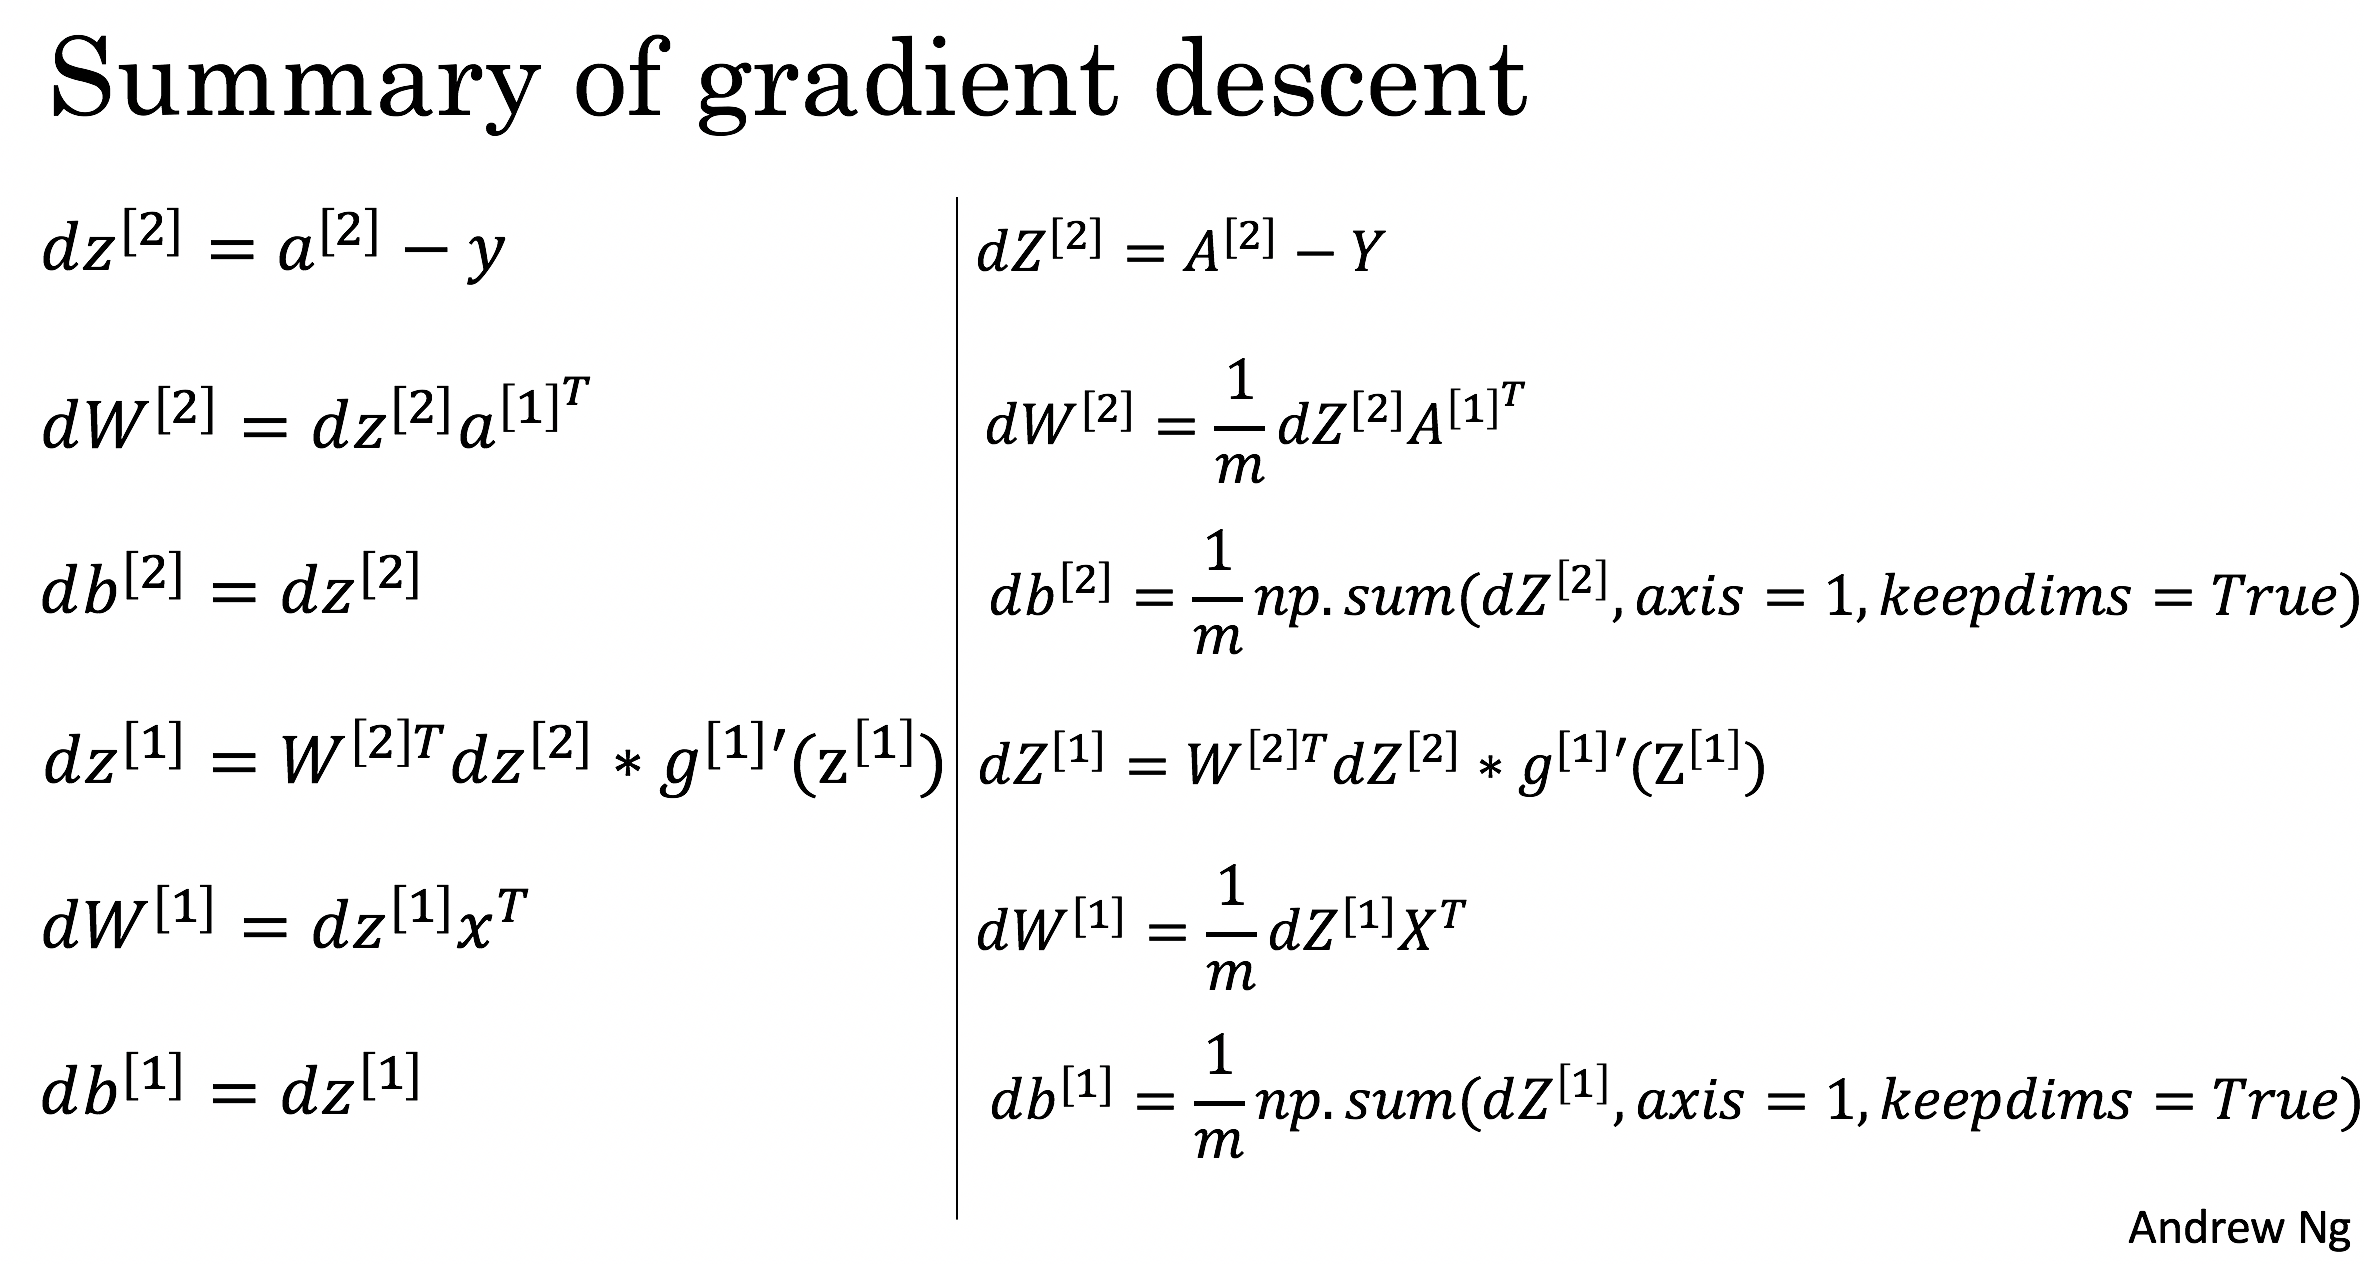
\includegraphics[width=0.9\textwidth]{course1/Backpropagation}
\end{center}
\caption{Back propagation}
\label{fig:Backpropagation}
\end{figure}

{\textbf {Tips}}:

    To compute dZ1 you'll need to compute $g^{[1]'}(Z^{[1]})$. Since $g^{[1]}(.)$ is the tanh activation function, if $a = g^{[1]}(z)$ then $g^{[1]'}(z) = 1-a^2$. So you can compute $g^{[1]'}(Z^{[1]})$ using `(1 - np.power(A1, 2))'.

\begin{minted}{python}
# GRADED FUNCTION: backward_propagation
def backward_propagation(parameters, cache, X, Y):
    """
    Implement the backward propagation using the instructions above.
    
    Arguments:
    parameters -- python dictionary containing our parameters 
    cache -- a dictionary containing "Z1", "A1", "Z2" and "A2".
    X -- input data of shape (2, number of examples)
    Y -- "true" labels vector of shape (1, number of examples)
    
    Returns:
    grads -- python dictionary containing your gradients with respect to different parameters
    """
    m = X.shape[1]
    
    # First, retrieve W1 and W2 from the dictionary "parameters".
    ### START CODE HERE ### (≈ 2 lines of code)
    W1 = parameters["W1"]
    W2 = parameters["W2"]
    ### END CODE HERE ###
        
    # Retrieve also A1 and A2 from dictionary "cache".
    ### START CODE HERE ### (≈ 2 lines of code)
    A1 = cache["A1"]
    A2 = cache["A2"]
    ### END CODE HERE ###
    
    # Backward propagation: calculate dW1, db1, dW2, db2. 
    ### START CODE HERE ### (≈ 6 lines of code, corresponding to 6 equations on slide above)
    dZ2 = A2-Y
    dW2 = np.dot(dZ2,A1.T)/m
    db2 = np.sum(dZ2,axis=1,keepdims=True)/m
    dZ1 = np.dot(W2.T,dZ2)*(1 - np.power(A1, 2))
    dW1 = np.dot(dZ1,X.T)/m
    db1 = np.sum(dZ1,axis=1,keepdims=True)/m
    ### END CODE HERE ###
    
    grads = {"dW1": dW1,
             "db1": db1,
             "dW2": dW2,
             "db2": db2}
    
    return grads
\end{minted}


{\textbf {Question}}: Implement the update rule. Use gradient descent. You have to use (dW1, db1, dW2, db2) in order to update (W1, b1, W2, b2).

{\textbf {General gradient descent rule}}: $ \theta = \theta - \alpha \frac{\partial J }{ \partial \theta }$ where $\alpha$ is the learning rate and $\theta$ represents a parameter.



\begin{minted}{python}
# GRADED FUNCTION: update_parameters
def update_parameters(parameters, grads, learning_rate = 1.2):
    """
    Updates parameters using the gradient descent update rule given above
    
    Arguments:
    parameters -- python dictionary containing your parameters 
    grads -- python dictionary containing your gradients 
    
    Returns:
    parameters -- python dictionary containing your updated parameters 
    """
    # Retrieve each parameter from the dictionary "parameters"
    ### START CODE HERE ### (≈ 4 lines of code)
    W1 = parameters["W1"]
    b1 = parameters["b1"]
    W2 = parameters["W2"]
    b2 = parameters["b2"]
    ### END CODE HERE ###

    # Retrieve each gradient from the dictionary "grads"
    ### START CODE HERE ### (≈ 4 lines of code)
    dW1 = grads["dW1"]
    db1 = grads["db1"]
    dW2 = grads["dW2"]
    db2 = grads["db2"]
    ## END CODE HERE ###
    
    # Update rule for each parameter
    ### START CODE HERE ### (≈ 4 lines of code)
    W1 = W1-learning_rate*dW1
    b1 = b1-learning_rate*db1
    W2 = W2-learning_rate*dW2
    b2 = b2-learning_rate*db2
    ### END CODE HERE ###
    
    parameters = {"W1": W1,
                  "b1": b1,
                  "W2": W2,
                  "b2": b2}
    
    return parameters
\end{minted}



\subsubsubsection{Integrate parts \ref{section4.1}, \ref{section4.2} and \ref{section4.3} in nn\_model()}

{\textbf {Question}}: Build your neural network model in nn\_model().

{\textbf {Instructions}}: The neural network model has to use the previous functions in the right order.


\begin{minted}{python}
# GRADED FUNCTION: nn_model
def nn_model(X, Y, n_h, num_iterations = 10000, print_cost=False):
    """
    Arguments:
    X -- dataset of shape (2, number of examples)
    Y -- labels of shape (1, number of examples)
    n_h -- size of the hidden layer
    num_iterations -- Number of iterations in gradient descent loop
    print_cost -- if True, print the cost every 1000 iterations
    
    Returns:
    parameters -- parameters learnt by the model. They can then be used to predict.
    """
    
    np.random.seed(3)
    n_x = layer_sizes(X, Y)[0]
    n_y = layer_sizes(X, Y)[2]
    
    # Initialize parameters, then retrieve W1, b1, W2, b2. Inputs: "n_x, n_h, n_y". Outputs = "W1, b1, W2, b2, parameters".
    ### START CODE HERE ### (≈ 5 lines of code)
    parameters = initialize_parameters(n_x, n_h, n_y)
    W1 = parameters["W1"]
    b1 = parameters["b1"]
    W2 = parameters["W2"]
    b2 = parameters["b2"]
    ### END CODE HERE ###
    
    # Loop (gradient descent)

    for i in range(0, num_iterations):
         
        ### START CODE HERE ### (≈ 4 lines of code)
        # Forward propagation. Inputs: "X, parameters". Outputs: "A2, cache".
        A2, cache =  forward_propagation(X, parameters)
        
        # Cost function. Inputs: "A2, Y, parameters". Outputs: "cost".
        cost = compute_cost(A2, Y, parameters)
 
        # Backpropagation. Inputs: "parameters, cache, X, Y". Outputs: "grads".
        grads = backward_propagation(parameters, cache, X, Y)
 
        # Gradient descent parameter update. Inputs: "parameters, grads". Outputs: "parameters".
        parameters = update_parameters(parameters, grads)
        
        ### END CODE HERE ###
        
        # Print the cost every 1000 iterations
        if print_cost and i % 1000 == 0:
            print ("Cost after iteration %i: %f" %(i, cost))

    return parameters
\end{minted}



{\textbf {Question}}: Use your model to predict by building predict().Use forward propagation to predict results.

{\textbf {Reminder}}: predictions = $y_{prediction} = \mathbb 1 \text{\{activation > 0.5\}} = \begin{cases}
      1 & \text{if}\ activation > 0.5 \\
      0 & \text{otherwise}
    \end{cases}$  
    
As an example, if you would like to set the entries of a matrix X to 0 and 1 based on a threshold you would do:\emph{ $X_{new} = (X > threshold)$}.


\begin{minted}{python}
# GRADED FUNCTION: predict
def predict(parameters, X):
    """
    Using the learned parameters, predicts a class for each example in X
    
    Arguments:
    parameters -- python dictionary containing your parameters 
    X -- input data of size (n_x, m)
    
    Returns
    predictions -- vector of predictions of our model (red: 0 / blue: 1)
    """
    
    # Computes probabilities using forward propagation, and classifies to 0/1 using 0.5 as the threshold.
    ### START CODE HERE ### (≈ 2 lines of code)
    A2, cache = forward_propagation(X, parameters)
    predictions = np.round(A2)
    ### END CODE HERE ###
    
    return predictions
\end{minted}


It is time to run the model and see how it performs on a planar dataset. Run the following code to test your model with a single hidden layer of  $n_h$  hidden units.

\begin{minted}{python}
# Build a model with a n_h-dimensional hidden layer
parameters = nn_model(X, Y, n_h = 4, num_iterations = 10000, print_cost=True)

# Plot the decision boundary
plot_decision_boundary(lambda x: predict(parameters, x.T), X, Y)
plt.title("Decision Boundary for hidden layer size " + str(4))
\end{minted}

The classification result of planar dataset is as follows:

\begin{figure}[h]
\begin{center}
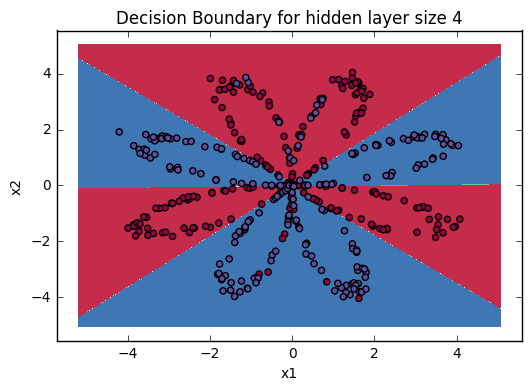
\includegraphics[width=0.6\textwidth]{course1/Decision_Boundary}
\end{center}
\caption{Decision Boundary for hidden layer size}
\label{fig:Decision_Boundary}
\end{figure}

\begin{minted}{python}
# Print accuracy
predictions = predict(parameters, X)
print ('Accuracy: %d' % float((np.dot(Y,predictions.T) + np.dot(1-Y,1-predictions.T))/float(Y.size)*100) + '%')

#Accuracy
Accuracy: 90%
\end{minted}


Accuracy is really high compared to Logistic Regression. The model has learnt the leaf patterns of the flower! Neural networks are able to learn even highly non-linear decision boundaries, unlike logistic regression.

Now, let's try out several hidden layer sizes.


\subsubsubsection{Tuning hidden layer size (optional/ungraded exercise)}

Run the following code. It may take 1-2 minutes. You will observe different behaviors of the model for various hidden layer sizes.

\begin{minted}{python}
# This may take about 2 minutes to run

plt.figure(figsize=(16, 32))
hidden_layer_sizes = [1, 2, 3, 4, 5, 20, 50]
for i, n_h in enumerate(hidden_layer_sizes):
    plt.subplot(5, 2, i+1)
    plt.title('Hidden Layer of size %d' % n_h)
    parameters = nn_model(X, Y, n_h, num_iterations = 5000)
    plot_decision_boundary(lambda x: predict(parameters, x.T), X, Y)
    predictions = predict(parameters, X)
    accuracy = float((np.dot(Y,predictions.T) + np.dot(1-Y,1-predictions.T))/float(Y.size)*100)
    print ("Accuracy for {} hidden units: {} %".format(n_h, accuracy))
\end{minted}

\begin{figure}
\begin{center}
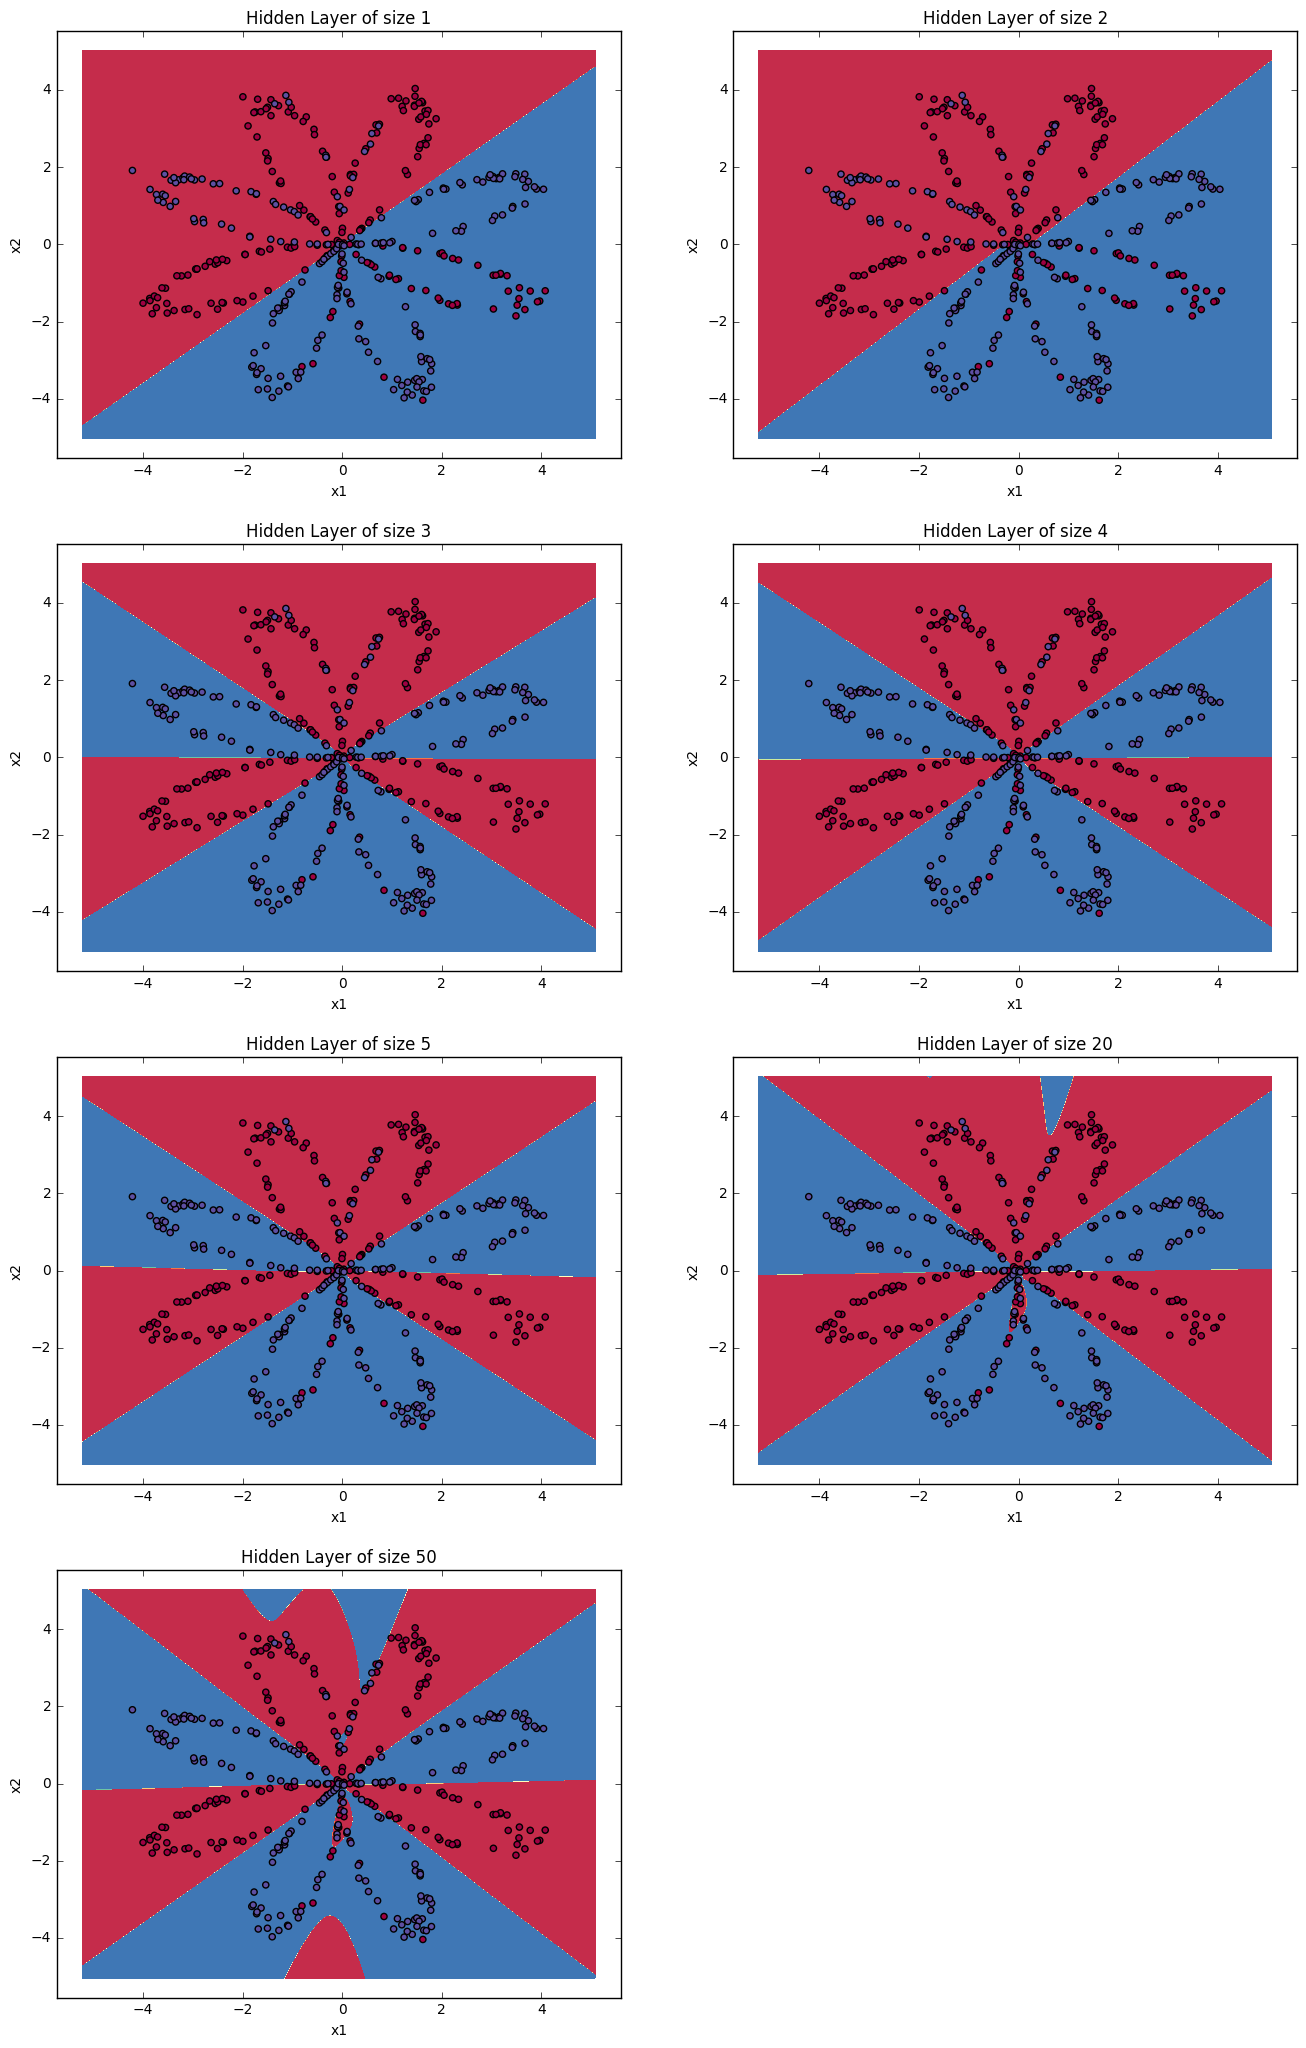
\includegraphics[width=\textwidth]{course1/various_hidden_layer_sizes}
\end{center}
\vspace{-0.5cm}
\caption{Different behaviors of the model for various hidden layer sizes}
\label{fig:various_hidden_layer_sizes}
\end{figure}


{\textbf {Interpretation}}:
\begin{itemize}
\item The larger models (with more hidden units) are able to fit the training set better, until eventually the largest models overfit the data.
\item The best hidden layer size seems to be around $n_h = 5$. Indeed, a value around here seems to fits the data well without also incurring noticable overfitting.
\item You will also learn later about regularization, which lets you use very large models (such as $n_h = 50$) without much overfitting.
\end{itemize}

{\color{blue}\textbf {
You've learnt to:
\begin{itemize}
\item Build a complete neural network with a hidden layer
\item Make a good use of a non-linear unit
\item Implemented forward propagation and backpropagation, and trained a neural network
\item See the impact of varying the hidden layer size, including overfitting.
\end{itemize}
}}

\clearpage
\subsubsection{Code of Neural Network With a Hidden Layer}
\begin{minted}{python}
# Package imports
import numpy as np
import matplotlib.pyplot as plt
from testCases_v2 import *
import sklearn
import sklearn.datasets
import sklearn.linear_model
from planar_utils import plot_decision_boundary, sigmoid, load_planar_dataset, load_extra_datasets

#matplotlib inline

np.random.seed(1) # set a seed so that the results are consistent

X, Y = load_planar_dataset()

# Visualize the data:
#plt.scatter(X[0, :], X[1, :], c=Y, s=40, cmap=plt.cm.Spectral);

shape_X = X.shape
shape_Y = Y.shape
m = shape_X[1]  # training set size

# Train the logistic regression classifier
#===================================
# clf = sklearn.linear_model.LogisticRegressionCV();
# clf.fit(X.T, Y.T);
# 
# # Plot the decision boundary for logistic regression
# plot_decision_boundary(lambda x: clf.predict(x), X, Y)
# plt.title("Logistic Regression")
# # Print accuracy
# LR_predictions = clf.predict(X.T)
# print ('Accuracy of logistic regression: %d ' %float((np.dot(Y,LR_predictions) +np.dot(1-Y,1-LR_predictions))/float(Y.size)*100) +'% ' + "(percentage of correctly labelled datapoints)")      
#===================================

# GRADED FUNCTION: layer_sizes
def layer_sizes(X, Y):
    """
    Arguments:
    X -- input dataset of shape (input size, number of examples)
    Y -- labels of shape (output size, number of examples)
    
    Returns:
    n_x -- the size of the input layer
    n_h -- the size of the hidden layer
    n_y -- the size of the output layer
    """
    n_x = X.shape[0] # size of input layer
    n_h = 4
    n_y = Y.shape[0]# size of output layer
    return (n_x, n_h, n_y)       
       

# GRADED FUNCTION: initialize_parameters
def initialize_parameters(n_x, n_h, n_y):
    """
    Argument:
    n_x -- size of the input layer
    n_h -- size of the hidden layer
    n_y -- size of the output layer
    
    Returns:
    params -- python dictionary containing your parameters:
                    W1 -- weight matrix of shape (n_h, n_x)
                    b1 -- bias vector of shape (n_h, 1)
                    W2 -- weight matrix of shape (n_y, n_h)
                    b2 -- bias vector of shape (n_y, 1)
    """
    
    np.random.seed(2) # we set up a seed so that your output matches ours although the initialization is random.
    
    W1 = np.random.randn(n_h,n_x) * 0.01
    b1 = np.zeros((n_h,1))
    W2 = np.random.randn(n_y,n_h)* 0.01
    b2 = np.zeros((n_y,1))
    
    assert (W1.shape == (n_h, n_x))
    assert (b1.shape == (n_h, 1))
    assert (W2.shape == (n_y, n_h))
    assert (b2.shape == (n_y, 1))
    
    parameters = {"W1": W1,
                  "b1": b1,
                  "W2": W2,
                  "b2": b2}
    
    return parameters


# GRADED FUNCTION: forward_propagation
def forward_propagation(X, parameters):
    """
    Argument:
    X -- input data of size (n_x, m)
    parameters -- python dictionary containing your parameters (output of initialization function)
    
    Returns:
    A2 -- The sigmoid output of the second activation
    cache -- a dictionary containing "Z1", "A1", "Z2" and "A2"
    """
    # Retrieve each parameter from the dictionary "parameters"
    W1 = parameters["W1"]
    b1 = parameters["b1"]
    W2 = parameters["W2"]
    b2 = parameters["b2"]
    
    # Implement Forward Propagation to calculate A2 (probabilities)
    Z1 = np.dot(W1,X)+b1
    A1 = np.tanh(Z1)
    Z2 = np.dot(W2,A1)+b2
    A2 = sigmoid(Z2)
    
    assert(A2.shape == (1, X.shape[1]))
    
    cache = {"Z1": Z1,
             "A1": A1,
             "Z2": Z2,
             "A2": A2}
    
    return A2, cache


# GRADED FUNCTION: compute_cost
def compute_cost(A2, Y, parameters):
    """
    Computes the cross-entropy cost given in equation (13)
    
    Arguments:
    A2 -- The sigmoid output of the second activation, of shape (1, number of examples)
    Y -- "true" labels vector of shape (1, number of examples)
    parameters -- python dictionary containing your parameters W1, b1, W2 and b2
    
    Returns:
    cost -- cross-entropy cost given equation (13)
    """
    
    m = Y.shape[1] # number of example

    # Compute the cross-entropy cost
    logprobs = np.multiply(np.log(A2),Y)+np.multiply(np.log(1-A2),1-Y)
    cost = - np.sum(logprobs)/m

#    use directly np.dot())
#    cost=-(np.dot(Y,np.log(A2.T))+np.dot(np.log(1-A2),(1-Y).T))/m
    
    cost = np.squeeze(cost)     # makes sure cost is the dimension we expect. 
                                # E.g., turns [[17]] into 17 
    
    return cost


# GRADED FUNCTION: backward_propagation
def backward_propagation(parameters, cache, X, Y):
    """
    Implement the backward propagation using the instructions above.
    
    Arguments:
    parameters -- python dictionary containing our parameters 
    cache -- a dictionary containing "Z1", "A1", "Z2" and "A2".
    X -- input data of shape (2, number of examples)
    Y -- "true" labels vector of shape (1, number of examples)
    
    Returns:
    grads -- python dictionary containing your gradients with respect to different parameters
    """
    m = X.shape[1]
    
    # First, retrieve W1 and W2 from the dictionary "parameters".
    W1 = parameters["W1"]
    W2 = parameters["W2"]
        
    # Retrieve also A1 and A2 from dictionary "cache".
    A1 = cache["A1"]
    A2 = cache["A2"]
    
    # Backward propagation: calculate dW1, db1, dW2, db2. 
    dZ2 = A2-Y
    dW2 = np.dot(dZ2,A1.T)/m
    db2 = np.sum(dZ2,axis=1,keepdims=True)/m
    dZ1 = np.dot(W2.T,dZ2)*(1 - np.power(A1, 2))
    dW1 = np.dot(dZ1,X.T)/m
    db1 = np.sum(dZ1,axis=1,keepdims=True)/m
    
    grads = {"dW1": dW1,
             "db1": db1,
             "dW2": dW2,
             "db2": db2}
    
    return grads


# GRADED FUNCTION: update_parameters
def update_parameters(parameters, grads, learning_rate = 1.2):
    """
    Updates parameters using the gradient descent update rule given above
    
    Arguments:
    parameters -- python dictionary containing your parameters 
    grads -- python dictionary containing your gradients 
    
    Returns:
    parameters -- python dictionary containing your updated parameters 
    """
    # Retrieve each parameter from the dictionary "parameters"
    W1 = parameters["W1"]
    b1 = parameters["b1"]
    W2 = parameters["W2"]
    b2 = parameters["b2"]

    # Retrieve each gradient from the dictionary "grads"
    dW1 = grads["dW1"]
    db1 = grads["db1"]
    dW2 = grads["dW2"]
    db2 = grads["db2"]
    
    # Update rule for each parameter
    W1 = W1-learning_rate*dW1
    b1 = b1-learning_rate*db1
    W2 = W2-learning_rate*dW2
    b2 = b2-learning_rate*db2
    
    parameters = {"W1": W1,
                  "b1": b1,
                  "W2": W2,
                  "b2": b2}
    
    return parameters



# GRADED FUNCTION: nn_model
def nn_model(X, Y, n_h, num_iterations = 10000, print_cost=False):
    """
    Arguments:
    X -- dataset of shape (2, number of examples)
    Y -- labels of shape (1, number of examples)
    n_h -- size of the hidden layer
    num_iterations -- Number of iterations in gradient descent loop
    print_cost -- if True, print the cost every 1000 iterations
    
    Returns:
    parameters -- parameters learnt by the model. They can then be used to predict.
    """
    
    np.random.seed(3)
    n_x = layer_sizes(X, Y)[0]
    n_y = layer_sizes(X, Y)[2]
    
    # Initialize parameters, then retrieve W1, b1, W2, b2. Inputs: "n_x, n_h, n_y". Outputs = "W1, b1, W2, b2, parameters".
    parameters = initialize_parameters(n_x, n_h, n_y)
    W1 = parameters["W1"]
    b1 = parameters["b1"]
    W2 = parameters["W2"]
    b2 = parameters["b2"]
    
    # Loop (gradient descent)

    for i in range(0, num_iterations):
         
        # Forward propagation. Inputs: "X, parameters". Outputs: "A2, cache".
        A2, cache =  forward_propagation(X, parameters)
        
        # Cost function. Inputs: "A2, Y, parameters". Outputs: "cost".
        cost = compute_cost(A2, Y, parameters)
 
        # Backpropagation. Inputs: "parameters, cache, X, Y". Outputs: "grads".
        grads = backward_propagation(parameters, cache, X, Y)
 
        # Gradient descent parameter update. Inputs: "parameters, grads". Outputs: "parameters".
        parameters = update_parameters(parameters, grads)
        
        
        # Print the cost every 1000 iterations
        if print_cost and i % 1000 == 0:
            print ("Cost after iteration %i: %f" %(i, cost))

    return parameters


#GRADED FUNCTION: predict
def predict(parameters, X):
    """
    Using the learned parameters, predicts a class for each example in X
    
    Arguments:
    parameters -- python dictionary containing your parameters 
    X -- input data of size (n_x, m)
    
    Returns
    predictions -- vector of predictions of our model (red: 0 / blue: 1)
    """
    
    # Computes probabilities using forward propagation, and classifies to 0/1 using 0.5 as the threshold.
    A2, cache = forward_propagation(X, parameters)
    predictions = np.round(A2)
    
    return predictions


# Build a model with a n_h-dimensional hidden layer
parameters = nn_model(X, Y, n_h = 4, num_iterations = 10000, print_cost=True)
plot_decision_boundary(lambda x: predict(parameters, x.T), X, Y)
plt.title("Decision Boundary for hidden layer size " + str(4))
print ('Accuracy: %d' % float((np.dot(Y,predictions.T) + np.dot(1-Y,1-predictions.T))/float(Y.size)*100) + '%')
\end{minted}


\clearpage